% Spikes n 1_(0,1/n) for n=1,2,4, with the curve 1/x through their outer corners.
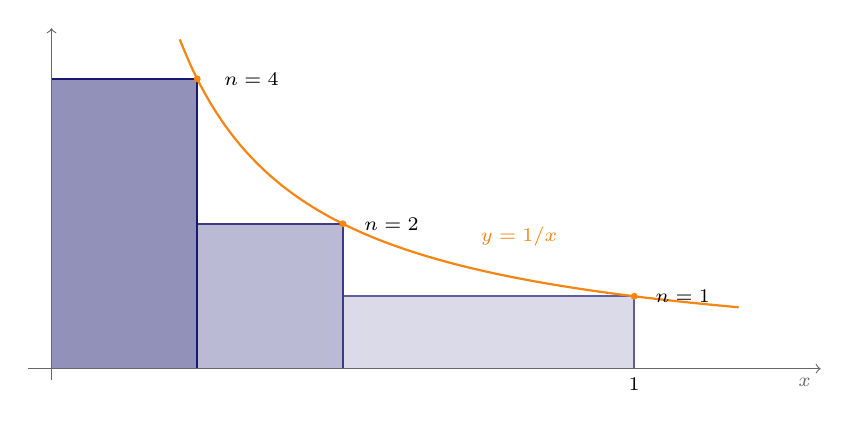
\begin{tikzpicture}[x=7.4cm,y=0.92cm]
  \fill[MidnightBlue!16] (0,0) rectangle (1,1);
  \draw[MidnightBlue!70,thick] (0,1) -- (1,1) -- (1,0);
  \fill[MidnightBlue!30] (0,0) rectangle (0.5,2);
  \draw[MidnightBlue!85,thick] (0,2) -- (0.5,2) -- (0.5,0);
  \fill[MidnightBlue!48] (0,0) rectangle (0.25,4);
  \draw[MidnightBlue,thick] (0,4) -- (0.25,4) -- (0.25,0);
  \draw[BurntOrange,thick,domain=0.22:1.18,samples=50,smooth] plot (\x,{1/\x});
  \fill[BurntOrange] (1,1) circle[radius=1.25pt];
  \fill[BurntOrange] (0.5,2) circle[radius=1.25pt];
  \fill[BurntOrange] (0.25,4) circle[radius=1.25pt];
  \draw[->,black!60] (-0.04,0) -- (1.32,0) node[below left,font=\scriptsize] {$x$};
  \draw[->,black!60] (0,-0.15) -- (0,4.7);
  \node[font=\scriptsize,anchor=north] at (1,0) {$1$};
  \node[font=\scriptsize,anchor=west] at (1.02,1) {$n=1$};
  \node[font=\scriptsize,anchor=west] at (0.52,2) {$n=2$};
  \node[font=\scriptsize,anchor=west] at (0.28,4) {$n=4$};
  \node[font=\scriptsize,BurntOrange,anchor=south west] at (0.72,1.55) {$y=1/x$};
\end{tikzpicture}
